\documentclass[12pt, a4paper]{article}

\usepackage[utf8]{inputenc}
\usepackage[framemethod=TikZ]{mdframed}
\usepackage[hidelinks]{hyperref}
\usepackage{mathtools, amssymb, amsmath, cleveref, fancyhdr, geometry, graphicx, float, subfigure, arydshln, url, setspace, framed, pifont, physics, ntheorem, utopia, tcolorbox}
%%% for coding %%%
\usepackage{listings}
\usepackage[ruled, vlined, linesnumbered]{algorithm2e}

\geometry{a4paper, left=2cm, right=2cm, bottom=2cm, top=2cm}

\pagestyle{fancy}
\fancyhead{}
\fancyhead[L]{\leftmark}
\fancyhead[R]{\rightmark}
\fancyfoot{}
\fancyfoot[C]{\thepage}
%\renewcommand{\headrulewidth}{0pt}
\renewcommand{\footrulewidth}{0pt}

\hypersetup{
	colorlinks = true,
	bookmarks = true,
	bookmarksnumbered = true,
	pdfborder = 001,
	linkcolor = blue
}

\definecolor{grey}{rgb}{0.49,0.38,0.29}
\definecolor{mygreen}{rgb}{0,0.6,0}


%%% for coding %%%
\lstset{basicstyle = \ttfamily\small,commentstyle = \color{mygreen}\textit, deletekeywords = {...}, escapeinside = {\%*}{*)}, frame = single, framesep = 0.5em, keywordstyle = \bfseries\color{blue}, morekeywords = {*}, emph = {self}, emphstyle=\bfseries\color{red}, numbers = left, numbersep = 1.5em, numberstyle = \ttfamily\small\color{grey},  rulecolor = \color{black}, showstringspaces = false, stringstyle = \ttfamily\color{purple}, tabsize = 4, columns = flexible}

\newcounter{index}[subsection]
\setcounter{index}{0}
\newenvironment*{df}[1]{\par\noindent\textbf{Definition \thesubsection.\stepcounter{index}\theindex\ (#1).}}{\par}

\newenvironment*{eg}[1]{\begin{framed}\par\noindent\textbf{Example \thesubsection.\stepcounter{index}\theindex\ #1} \par}{\par\end{framed}}

\newenvironment*{thm}[1]{\begin{tcolorbox}\par\noindent\textbf{Theorem \thesubsection.\stepcounter{index}\theindex\ #1} \par}{\par\end{tcolorbox}}

\newenvironment*{cor}[1]{\par\noindent\textbf{Corollary \thesubsection.\stepcounter{index}\theindex\ #1}}{\par}
\newenvironment*{lem}[1]{\par\noindent\textbf{Lemma \thesubsection.\stepcounter{index}\theindex\ #1}}{\par}
\newenvironment*{ax}[1]{\par\noindent\textbf{Axiom \thesubsection.\stepcounter{index}\theindex\ #1}}{\par}
\newenvironment*{prop}[1]{\par\noindent\textbf{Proposition \thesubsection.\stepcounter{index}\theindex\ #1}}{\par}
\newenvironment*{conj}[1]{\par\noindent\textbf{Conjecture \thesubsection.\stepcounter{index}\theindex\ #1}}{\par}
\newenvironment*{nota}{\par\noindent\textbf{Notation \thesubsection.\stepcounter{index}\theindex.}}{\par}

\newcounter{nprf}[subsection]
\setcounter{nprf}{0}
\newenvironment*{prf}{\par\indent\textbf{\textit{Proof \stepcounter{nprf}\thenprf.}}}{\hfill$\blacksquare$\par}
\newenvironment*{dis}{\par\indent\textbf{\textit{Disproof \stepcounter{nprf}\thenprf.}}}{\hfill$\blacksquare$\par}
\newenvironment*{sol}{\par\indent\textbf{\textit{Solution \stepcounter{nprf}\thenprf.}}\par}{\hfill{$\square$}\par}

\newtheorem*{hint}{Hint.}
\newtheorem*{rmk}{Remark.}
\newtheorem*{ext}{Extension.}

\linespread{1.25}

\title{\textbf{This is a title}}
\author{Jiuru Lyu}
\date{\today}

\def\Z{{\mathbb{Z}}}
\def\R{{\mathbb{R}}}
\def\C{{\mathbb{C}}}
\def\Q{{\mathbb{Q}}}
\def\E{{\mathbb{E}}}
\def\d{{\mathrm{d}}}
\def\float{\texttt{float}}
\def\flt{\texttt{float}}
\def\Inf{\texttt{Inf}}
\def\NaN{\texttt{NaN}}
\def\epsilon{\varepsilon}
\def\emptyset{\varemptyset}


\begin{document}
\maketitle

\tableofcontents

\newpage
\section{Floating Point Numbers}
\subsection{Binary Representation}
\begin{df}{Binary}
	$0$ and $1$; on and off.	
\end{df}
\begin{eg}{Represent Numbers in Base-2}
	\par Consider $13=1(10)+3(1)=1(10)+3(10^0)$ in base-10. It can be converted into base-2 by decomposing $13$ as $1(2^3)+1(2^2)+0(2^1)+1(2^0)$.
\end{eg}
\begin{eg}{Fractions in Base-2}
	\[\dfrac{7}{16}=\dfrac{1}{16}(7)=\qty(2^{-4})\qty(2^2+2^1+2^0)=2^{-2}+2^{-3}+2^{-4}.\]
\end{eg}
\begin{eg}{Repeating Fractions in Base-2}
	\[\begin{aligned}\dfrac{1}{5}=\dfrac{1}{8}+\epsilon_1\quad&\Longrightarrow\quad\epsilon_1=\dfrac{1}{5}-\dfrac{1}{8}=\dfrac{8-5}{(5\times8)}=\dfrac{3}{40}\\\epsilon_1=\dfrac{3}{3(16)}+\epsilon_2\quad&\Longrightarrow\quad\cdots\end{aligned}\] Repeating the steps above, we would finally get \[\dfrac{1}{5}=\dfrac{1}{8}+\dfrac{1}{16}+\dfrac{1}{128}+\dfrac{1}{256}+\cdots\]
\end{eg}
\begin{thm}{}
	Let $n\in\Z$ and $n\geq1$, then \[\sum_{k=0}^{n-1}2^k=2^{n-1}+2^{n-2}+\cdots+2^0=2^n-1.\]	
\end{thm}
\subsection{Integers in Computers}
\begin{df}{Storing Integers}
	\texttt{unit8} stands for unsigned integers and \texttt{int8} stands for signed integers. 
	\begin{rmk} The $8$ here represents $8$ bits. It is a measure of how much storage (how many $0$s or $1$s).\end{rmk}
	\[\begin{aligned}
	\begin{tabular}{|c|c|c|c|c|c|c|c|}
		\hline
		\ $b_7$&$b_6$\ &\ $b_5$&$b_4$\ &\ $b_3$&$b_2$\ &\ $b_1$&\ $b_0$\\
		\hline
	\end{tabular}&\\
	\begin{tabular}{ccccccccc}	
		unsigned: &$2^7$&$2^6$&$2^5$&$2^4$&$2^3$&$2^2$&$2^1$&$2^0$\\
		signed:   &$-2^7$&$2^6$&$2^5$&$2^4$&$2^3$&$2^2$&$2^1$&$2^0$
	\end{tabular}&
	\end{aligned}\]
\end{df}
\begin{eg}{}
	\[\texttt{unit8}(13)=00001101\] Since $-13=1(-2^7)+1(2^6)+1(2^5)+1(2^4)+0(2^3)+0(2^2)+1(2^1)+1(2^0)$, we have \[\texttt{int8}(-13)=11110011\]
\end{eg}
\begin{rmk}
	Largest and Smallest Integers: \[\begin{aligned}\textnormal{\texttt{uint8}}(x_L)&=11111111\quad\Longrightarrow x_L=2^7+2^6+\cdots+2^0=2^8-1=255\\\textnormal{\texttt{uint8}}(x_S)&=00000000\quad\Longrightarrow x_S=0(2^7)+0(2^6)+\cdots+0(2^0)=0\\\textnormal{\texttt{int8}}(x_L)&=01111111\quad\Longrightarrow x_L=0(-2^7)+2^6+\cdots+2^0=2^7-1=127\\\textnormal{\texttt{int8}}(x_S)&=100000000\quad\Longrightarrow x_S=1(-2^7)+0(2^6)+\cdots+0(2^0)=-128\end{aligned}\]	
\end{rmk}
\subsection{Representation of Floating Point Numbers}
\begin{df}{Normalized Scientific Notation}
	Only $1$ digit (non-zero) to the left of the decimal point.	
\end{df}
\begin{eg}{}
	\[\begin{aligned}123.456\times10^7&\\12.3456\times10^8&\\1.23456\times10^9&\rightarrow\text{normalized}\end{aligned}\]	
\end{eg}
\begin{df}{Anatomy of Floating Point Numbers}
	A floating point number, $\texttt{float}(x)$, consists of three parts: $s(x)$ (sign bit), $e(x)$ (exponent bits), and $f(x)$ (fraction bits).
\end{df}
\begin{df}{Precision}
	Precision is defined by the number 	of bits per part:
	\begin{center}\begin{tabular}{c|c|c|c|c}
	&$s(x)$&$e(x)$&$f(x)$&total\\\hline
	double precision (DP)&$1$&$11$&$52$&$64$\\
	single precision (SP)&$1$&$8$&$23$&$32$\\
	half precision (HP)&$1$&$5$&$10$&$16$\\
	\end{tabular}\end{center}
	\begin{rmk}The less bits the float point number has, the less storage it requires and faster computation it performs, but more error introduces.\end{rmk}
\end{df}
\begin{df}{Floating Point Number}
	\begin{equation}\label{eq1}\texttt{float}(x)=(-1)^{s(x)}\qty(1+\dfrac{f(x)}{2^\text{\# of fraction bits}})2^{E(x)},\end{equation} where $E(x)$ is called the \textit{unbiased exponent} because it is centered about $0$ and is calculated through the $e(x)$, the \textit{biased exponent} because it can only be non-negative integers, by the following formula: \[E(x)=e(x)-\qty(2^{\text{\# of exponent bits}-1}-1).\]	
	\begin{rmk}
		Eq. (\ref{eq1}) is in normalized scientific notation because the largest number $f(x)$ can represent is $2^\textnormal{\# of fraction bits}-1$. Hence, \[1+\dfrac{f(x)}{2^\textnormal{\# of fraction bits}}<2,\] and thus there will be only $1$ digit in front of the decimal point.
	\end{rmk}
\end{df}
\begin{eg}{Formula for a Floating Point Number in Double Precision (DP)}
	\[\texttt{float}_\text{DP}(x)=(-1)^{s(x)}\qty(1+\dfrac{f(x)}{2^{52}})2^{e(x)-1023}.\]	
\end{eg}
\begin{eg}{Converting DP into Decimal}
	\par Suppose a DP floating number is stored as $s(x)=0$, $e(x)=10000000011,$ and $f(x)=0100100\cdots0$. Find its representation in decimal base-10.
	\begin{sol}
		$e(x)=10000000011=2^{10}+2^{1}+2^{0}$ and $f(x)=0100100\cdots0=2^{50}+2^{47}$. Then, the unbiased exponent $E(x)=e(x)-1023=2^{10}+2^1+2^0-\qty(2^{10}-1)=4$. So, \[\begin{aligned}\texttt{float}_\text{DP}(x)&=(-1)^{s(x)}+\qty(1+\dfrac{f(x)}{2^{52}})2^{E(x)}\\&=(-1)^0\qty(1+\dfrac{2^{50}+2^{47}}{2^{52}})2^4\\&=\qty(1+2^{-2}+2^{-5})2^4\\&=2^4+2^2+2^{-1}\\&=16+4+0.5=20.5\end{aligned}\]
	\end{sol}
\end{eg}
\begin{eg}{Converting Value to DP}
	\par Suppose a number in base-10 is $-10.75$. Find its representation of floating point number under DP.
	\begin{sol}
	We have
		\[\begin{aligned}\texttt{value}(x)=-10.75&=(-1)(10+0.75)\\&=(-1)\qty(2^3+2^1+2^{-1}+2^{-2})\\&=(-1)\qty(1+2^{-2}+2^{-4}+2^{-5})2^3\quad\qty\Big[\text{In normalized scientific notation}]\\&=(-1)^1\qty(1+\dfrac{2^{50}+2^{48}+2^{47}}{2^{52}})2^{1026-1023}\\&=(-1)^1\qty(1+\dfrac{2^{50}+2^{48}+2^{47}}{2^{52}})2^{2^{10}+2^{1}-1023}\end{aligned}\]So, we have $s(x)=1$, $e(X)=10000000010$, and $f(x)=010110\cdots0$.
	\end{sol}
\end{eg}
\begin{thm}{Some Special Rules}
	\begin{enumerate}
		\item The formula \[\texttt{value}(x)=(-1)^{s(x)}+\qty(1+\dfrac{f(x)}{2^{52}})2^{e(x)-1023}\] only holds when $0<e(x)<2^{11}-1$ or $00\cdots01<e(x)<11\cdots10$.
		\item If $e(x)=11\cdots1$, then it encodes special numbers.
		\item If $e(x)=00\cdots0$: 
		\begin{itemize}
			\item If $f(x)=00\cdots0$, then $\texttt{value}(x)=0$.
			\item If $f(x)>0$, it encodes a \textit{denormalized floating point number}: \[\texttt{value}(x)=(-1)^{s(x)}\qty(0+\dfrac{f(x)}{2^{52}})2^{-1022}.\] This denormalized floating point number is more precise when describing really small things. 
		\end{itemize}
	\end{enumerate}
\end{thm}
\begin{df}{Machine Epsilon/$\epsilon_\text{WP}$}
	Let ``WP'' stands for the working precision (DP/SP/HP/etc.). The \textit{machine epsilon}, denoted as $\epsilon_\text{WP}$, is the gap between $1$ and the next largest floating point number. Equivalently, it can be viewed as the smallest possible non-zero value of $\dfrac{f(x)}{2^\text{number of fraction bits}}$. So, $\epsilon_\text{DP}=2^{-52}$, $\epsilon_\text{SP}=2^{-23}$, and $\epsilon_\text{HP}=2^{-10}$.
\end{df}
\begin{df}{Special Numbers}
	\begin{enumerate}
		\item $\pm0$: when $s(x)=\pm1$ and $e(x)=f(x)=0$.
		\item $\pm\Inf$
		\item $\NaN$: not-a-number
	\end{enumerate}	
\end{df}
\begin{df}{Floating Point Arithmetic}
	\begin{enumerate}
		\item The set of real numbers, $\R$, is closed under arithmetic operations.
		\item The set of all WP floating point numbers, however, is not closed under arithmetic operations. For example, $\texttt{float}_\text{DP}(x)=\texttt{float}_\text{DP}(y)=2^{52}+1$, but $xy=2^{104}+\epsilon$ cannot be represented using DP. 
		\item Suppose $x$ and $y$ are floating point numbers, then $x\oplus y=\texttt{float}(x+y)$ and $x\otimes y=\texttt{float}(xy)$. Consider \texttt{float} as a rounding process, we can also define subtraction and division of floating point numbers. 
	\end{enumerate}	
\end{df}
\begin{eg}{}
	Assume we are only allowed three significant digits (in Base-10) in a computer. Suppose $x=1.23\times10^4$ and $y=6.54\times10^3$. Find $x\oplus y=\texttt{float}(x+y)$.
	\begin{sol}
		\[\begin{aligned}x\oplus y&=\texttt{float}(x+y)\\&=\texttt{float}(1.23\times10^4+6.54\times10^3)\\&=\texttt{float}(1.23\times10^4+0.654\times10^3)\\&=\texttt{float}(1.884\times10^4)\\&=1.88\times10^4.\end{aligned}\]
	\end{sol}
\end{eg}

\subsection{Errors}
\begin{df}{Errors We May See}
	\begin{enumerate}
		\item \textit{Overflow}: The exponent is too large. This means $\qty|x|$ is large and the computer will represent it as $\pm\Inf.$ Note: In DP, $x_\text{large}=\qty(2-2^{-52})\times2^{1023}\approx1.798\times10^{308}$. This number is referred as \texttt{realmax} in MATLAB.
		\item \textit{Underflow}: Large negative exponent. This means $\qty|x|$ is tiny and the computer will represent it as $\pm0$. Note: In SP, $x_\text{small}\approx2.225\times10^{-53}$ and is referred as \texttt{realmin} in MATLAB.
		\item \textit{Roundoff error}: cutoff or round at some point. 
	\end{enumerate}	
	Note that sometimes we are encounter the catastrophic cancellation, meaning the subtraction leads to our loss of significance or information. In this case, it is different from underflow error or roundoff error.
\end{df}
\begin{eg}{Catastrophic Cancellation/Loss of Significance Due to Subtraction}
	\[\begin{aligned}x&=3.141592920353983\approx\dfrac{355}{113}&\quad16\text{ digits}\\y&=3.141592653589794\approx\pi&\quad16\text{ digits}\\x-y&=0.000000266764189&\quad9\text{ digits}\end{aligned}\]
\end{eg}
\begin{df}{Relative Error}
	Let $z\in\R$. The relative error between $\float(z)$ and $z$ is denoted as $\mu$ and \[\mu=\dfrac{\float(z)-z}{z}\]\[\float(z)=z(1+\mu),\] where we know \[\qty|\mu|\leq\dfrac{\epsilon_\text{WP}}{2}.\]
\end{df}
\begin{eg}{Propagation of Errors}
	There are two major sources of errors: storing number and arithmetics. \par Consider a computer only allow $3$ significant figures. Then $\epsilon_\text{WP}=0.01$.\par Consider $x=\dfrac{1}{3}$, $y=\dfrac{8}{7}$, and $x+y=\dfrac{31}{21}$. Then, \[\float(x)=0.333=3.33\times10^{-1}=x\qty(1+\mu_x).\] Solving for $\mu_x$: \[\begin{aligned}\dfrac{333}{1000}&=\dfrac{1}{3}\qty(1+\mu_x)\\\mu_x&=\dfrac{999}{1000}-1=\dfrac{-1}{1000}=-0.001\end{aligned}\] Note that $\qty|\mu_x|=0.01<\dfrac{\epsilon_\text{WP}}{2}$. Similarly, we can solve  $\float(y)=1.14\times10^0=y\qty(1+\mu_y)$ for $\qty|\mu_y|=0.0025$. Now, consider the floating point addition \[\begin{aligned}x\oplus y&=\flt(\flt(x)+\flt(y))\\&=\flt(3.33\times10^{-1}+1.14\times10^0)\\&=\flt(1.473\times10^0)\\&=1.47\times10^0.\end{aligned}\] Also, solve $x\oplus y=(x+y)\qty(1+\mu_a)$ for $\qty|\mu_a|=0.0042$. Note that \[\qty|\mu_x|+\qty|\mu_y|=0.0035<0.0042=\qty|\mu_a|.\] This is called the propagation of error. 
\end{eg}
\begin{eg}{Plotting Exponentials Using Factored and Expanded Forms}
	Consider $p(x)=(1-x)^{10}$ and its expanded form.
	Plot them to see which is better. 
	\begin{lstlisting}[language = Matlab, title = {Example 1.4.5}]
	%% Defining the Functions
	p_1 = @(x) (1-x).^10;
	p_2 = @(x) x.^10-10*x.^9+45*x.^8-120*x.^7+210*x.^6-252*x.^5+...
			210*x.^4-120*x.^3+45*x.^2-10*x+1;
	%% Ploting the Functions
	x = linspace(0, 2, 100);
	plot(x, p_1(x))
	hold on
	plot(x, p_2(x))
	legend("Factor", "Expanded")
	%% Zooming In
	y = linspace(0.99, 1.01, 100);
	hold off
	plot(y, p_1(y))
	hold on
	plot(y, p_2(y))
	legend("Factor", "Expanded")
	\end{lstlisting}
	\begin{figure}[H]\centering
	\subfigure[Plotting Functions]{\label{plottingFuc}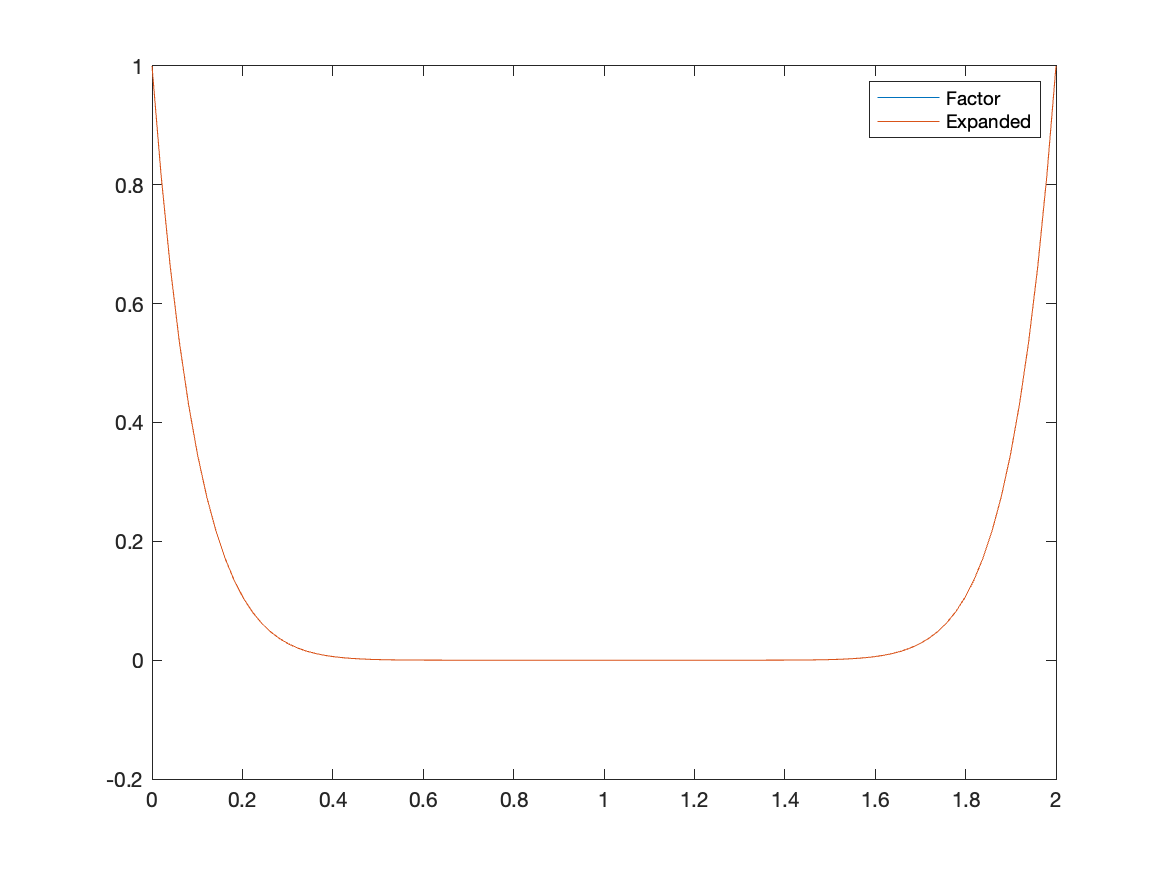
\includegraphics[width=0.48\textwidth]{figs/Ex2_3_1_Ploting_Functions}}
	\hfill
	\subfigure[Zooming In]{\label{zoomingIn}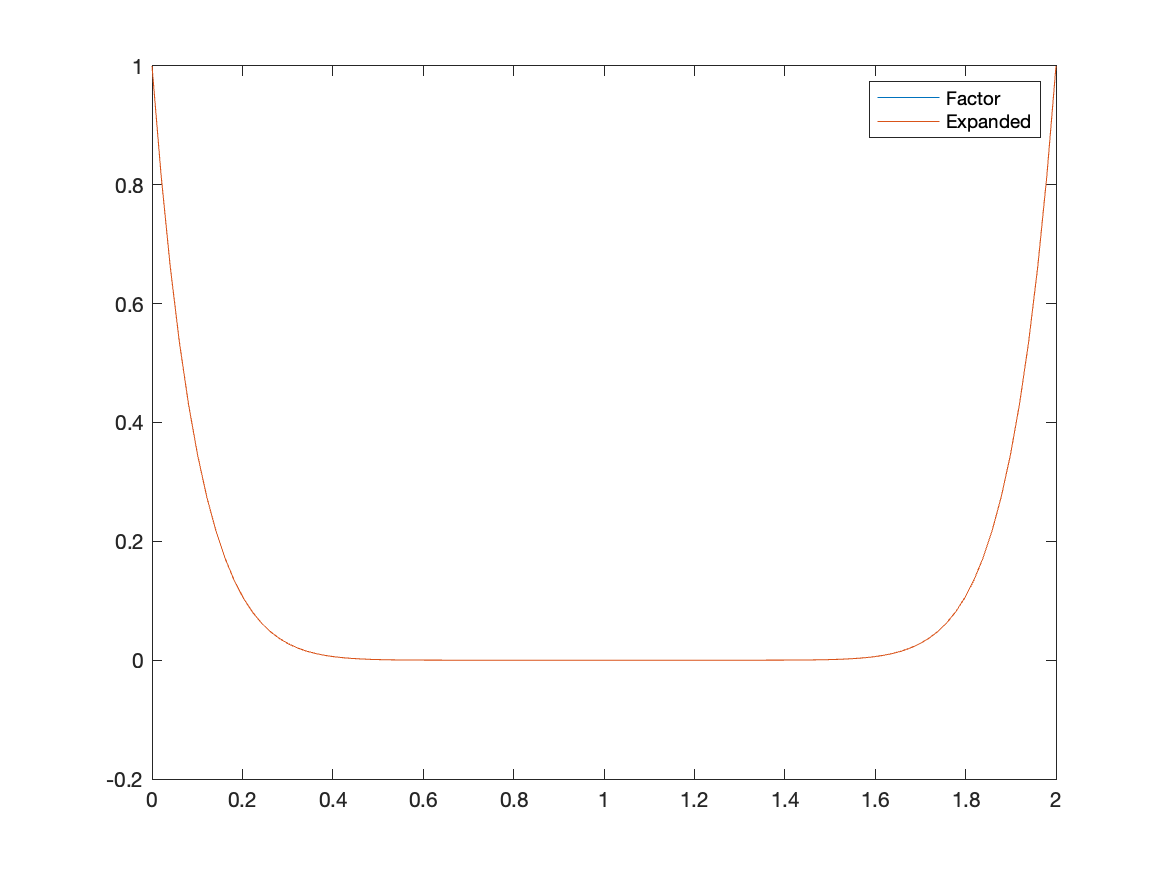
\includegraphics[width=0.5\textwidth]{figs/Ex2_3_1_Ploting_Functions}}\end{figure}
	It seems that the two functions are the same (Fig \ref{plottingFuc}); however if we zooming in (Fig \ref{zoomingIn}), the expanded version introduces more error than the factored version because the expanded version requires more arithmetical operations in it. 
	\end{eg}





\begin{algorithm}
\caption{Bisection Algorithm}
\SetKwData{In}{\rmfamily\textbf{in}}\SetKwData{To}{\rmfamily\textbf{to}}\SetKwData{And}{\rmfamily{\textbf{and}}}\SetKwData{Or}{\rmfamily{\textbf{or}}}\SetKwData{Stop}{\rmfamily{\textbf{stop}}}\SetKwData{Break}{\rmfamily{\textbf{break}}}
\SetKwComment{Comment}{/* }{ */}
\DontPrintSemicolon
\KwIn{$a,b,M,\delta,\epsilon$\;$u\leftarrow f(a)$\;$b\leftarrow f(b)$\;$e\leftarrow b-a$}
\KwOut{output}
\BlankLine
\Begin{
	\If{$\text{sign}(u)=\text{sign}(v)$}{\Stop}
	\For{k=1 \To M}{
		$e\leftarrow e/2$\;
		$c\leftarrow a+e$\;
		$w\leftarrow f(c)$\;
		\Return $k,c,w,e$\;
		\If{$|e|<\delta$\Or$|w|<\epsilon$}{\Stop}
		\eIf{$\text{sign}(u)\neq=\text{sign}(v)$}{
			$b\leftarrow c$\;
			$v\leftarrow w$\;
		} {
			$a\leftarrow c$\;
			$u\leftarrow w$\;
		}
	}
}
\end{algorithm}
\end{document}